\lstset{frame=tb,
	language=C++,
	aboveskip=3mm,
	belowskip=3mm,
	showstringspaces=false,
	columns=flexible,
	basicstyle={\small\ttfamily},
	numbers=none,
	numberstyle=\tiny,
	breaklines=true,
	breakatwhitespace=true,
	tabsize=3}

\chapter{Verificarea formală a problemei}

\section{Implementarea algoritmului}
    Implementarea algoritmului propriu-zis care rezolvă problema a fost primul și cel mai ușor pas.\par
    Am început prin crearea unei bucle care la fiecare pas alegea bancnota optimă, o adăuga în secvența de 
    bancnote considerată soluție și o scădea din sumă, fiind un algoritm tipic metodei Greedy.
    \begin{lstlisting}
    var rest:= sum;
    solution:= [0, 0, 0, 0, 0, 0];
    while (0 < rest)
        decreases rest 
        {
        index:= maxBanknote(rest);
        var banknote:= power(2, index);
        solution:= addValueToIndex(solution,1,index);
        rest:= rest - banknote;
    }
    \end{lstlisting}

    Acest algoritm era suficient pentru a rezolva problema, dar nu era suficient pentru a demonstra că soluția produsă este optimă.\par
    Considerăm o soluție optimă soluția de cost minim, costul fiind numărul de bancnote.
    
\section{Demonstrarea optimalității}
    \subsection{Schema verificării}
    \vspace{1cm}
        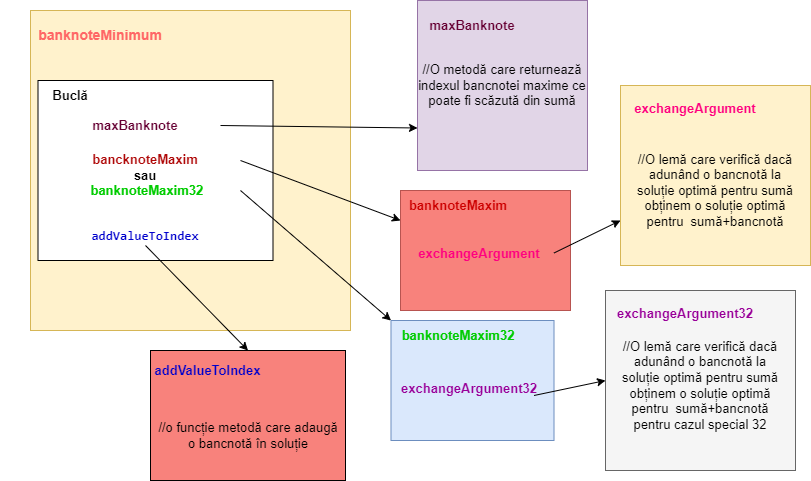
\includegraphics[width=0.9\textwidth]{verification_schema.png}\par
    În schema de mai sus am exemplificat modul în care funcțiile, lemele și metodele se apelează una pe cealaltă pentru a demonstra faptul că soluția găsită este soluție optimă.\par

    \subsection{Pașii verificării}
    
    
    \subsection{Detalii de implementare}
    //exemple cod pentru cele mai importante: exchange argument32, banknoteMaxim32, maxBanknote , metoda principala

\section{Posibile îmbunătățiri ???}


